%%%%%%%%%%%%%%%%%%%%%%%%%%%%%%%%%%%%%%%%%%%%%%%%%%%%%%%%%%%%%%%%%%%%%%%%%%%%%%%%
\section{On Efficiency}
\ifdefined\ishandout
{
    \frame{
        \tableofcontents[currentsection]
    }
}
\else
{   
	
    \usebackgroundtemplate{
        \vbox to \paperheight{\vfil\hbox to \paperwidth{\hfill
\includegraphics[width=.7\paperwidth]{efficiency/spread.jpeg}}}
    }
    \frame{
        \frametitle{Fitting Ressources -- avoiding Contention}
        \begin{mdframed}[tikzsetting={draw=white,fill=white,fill opacity=0.8,
                line width=0pt},backgroundcolor=none,leftmargin=0,
            rightmargin=150,innertopmargin=4pt,roundcorner=10pt]
            \tableofcontents[currentsection,sections={1-4},hideothersubsections]
        \end{mdframed}
        \vspace{1em}
        {\tiny "spread - 2026"; pencil and charcoal C. Meesters -- CC-BY-4.0}
    }
}
\fi

%%%%%%%%%%%%%%%%%%%%%%%%%%%%%%%%%%%%%%%%%%%%%%%%%%%%%%%%%%%%%%%%%%%%%%%%%%%%%%%%
\begin{frame}
    \frametitle{This is HPC - Efficiency matters!}
    \begin{hint}[Assumption]
    	\emph{All} data analysis requires heterogeneous resources!
    \end{hint}
    \begin{columns}
    	\begin{column}{0.5\textwidth}
    		Imagine a sequential workflow on one node!
    	\end{column}
    	\begin{column}{0.5\textwidth}
    		\only<1>{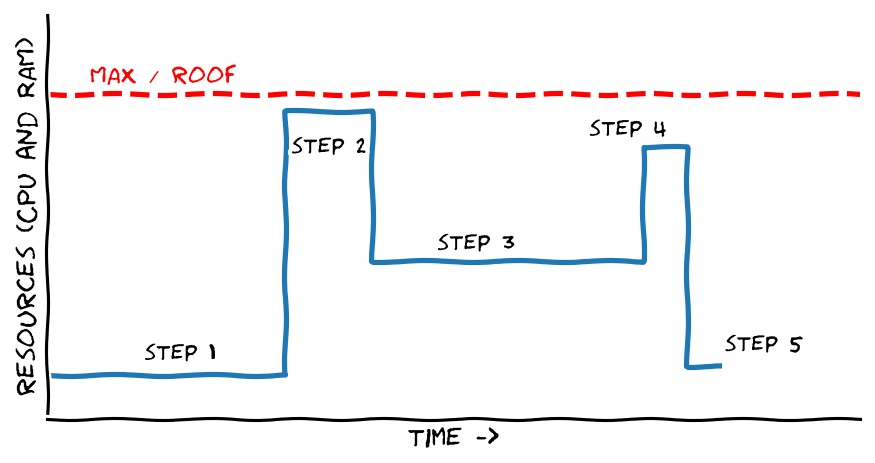
\includegraphics[width=0.9\textwidth]{efficiency/pipeline_xkcd}}
    		\only<2>{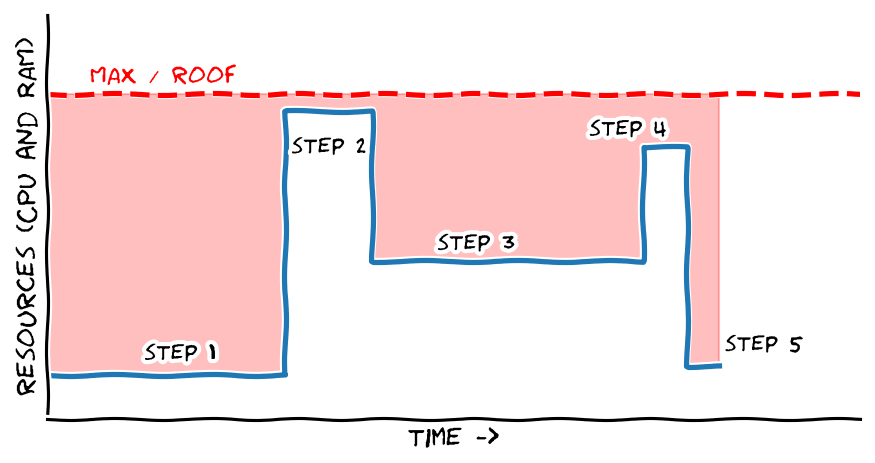
\includegraphics[width=0.9\textwidth]{efficiency/pipeline_xkcd_waste}\\
    		Then $\curvearrowright \int \mathrm{"red"} = \mathrm{"unused resources"}$} 
    	\end{column}
    \end{columns}
\end{frame}

%%%%%%%%%%%%%%%%%%%%%%%%%%%%%%%%%%%%%%%%%%%%%%%%%%%%%%%%%%%%%%%%%%%%%%%%%%%%%%%%
\begin{frame}
	\frametitle{Considerations}
	
\begin{columns}
		\begin{column}{0.5\textwidth}
	\emph{Some} clusters enforce
	\begin{itemize}
		\item to run an analysis on one node (no shepherd on the login!)
		\item Or disallow workflow managers altogether. 
	\end{itemize}
	We can estimate the waste with $\mathrm{R_1}$ being the runtime of \emph{one} pipeline and $\mathrm{E_{app}}$ the apparent efficiency and $\mathrm{N_{samples}}$ the number of samples or pipelines to be:
	\begin{center}
		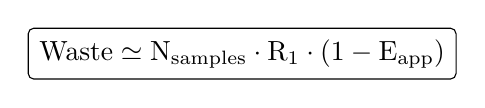
\begin{tikzpicture}
			\node[draw, rounded corners=2pt, line width=0.4pt, inner sep=4pt] {$\mathrm{Waste} \simeq \mathrm{N_{samples}} \cdot \mathrm{R_1} \cdot \mathrm{(1} - \mathrm{E_{app})}$};
		\end{tikzpicture}
	\end{center}
		\end{column}
		\begin{column}{0.5\textwidth}
			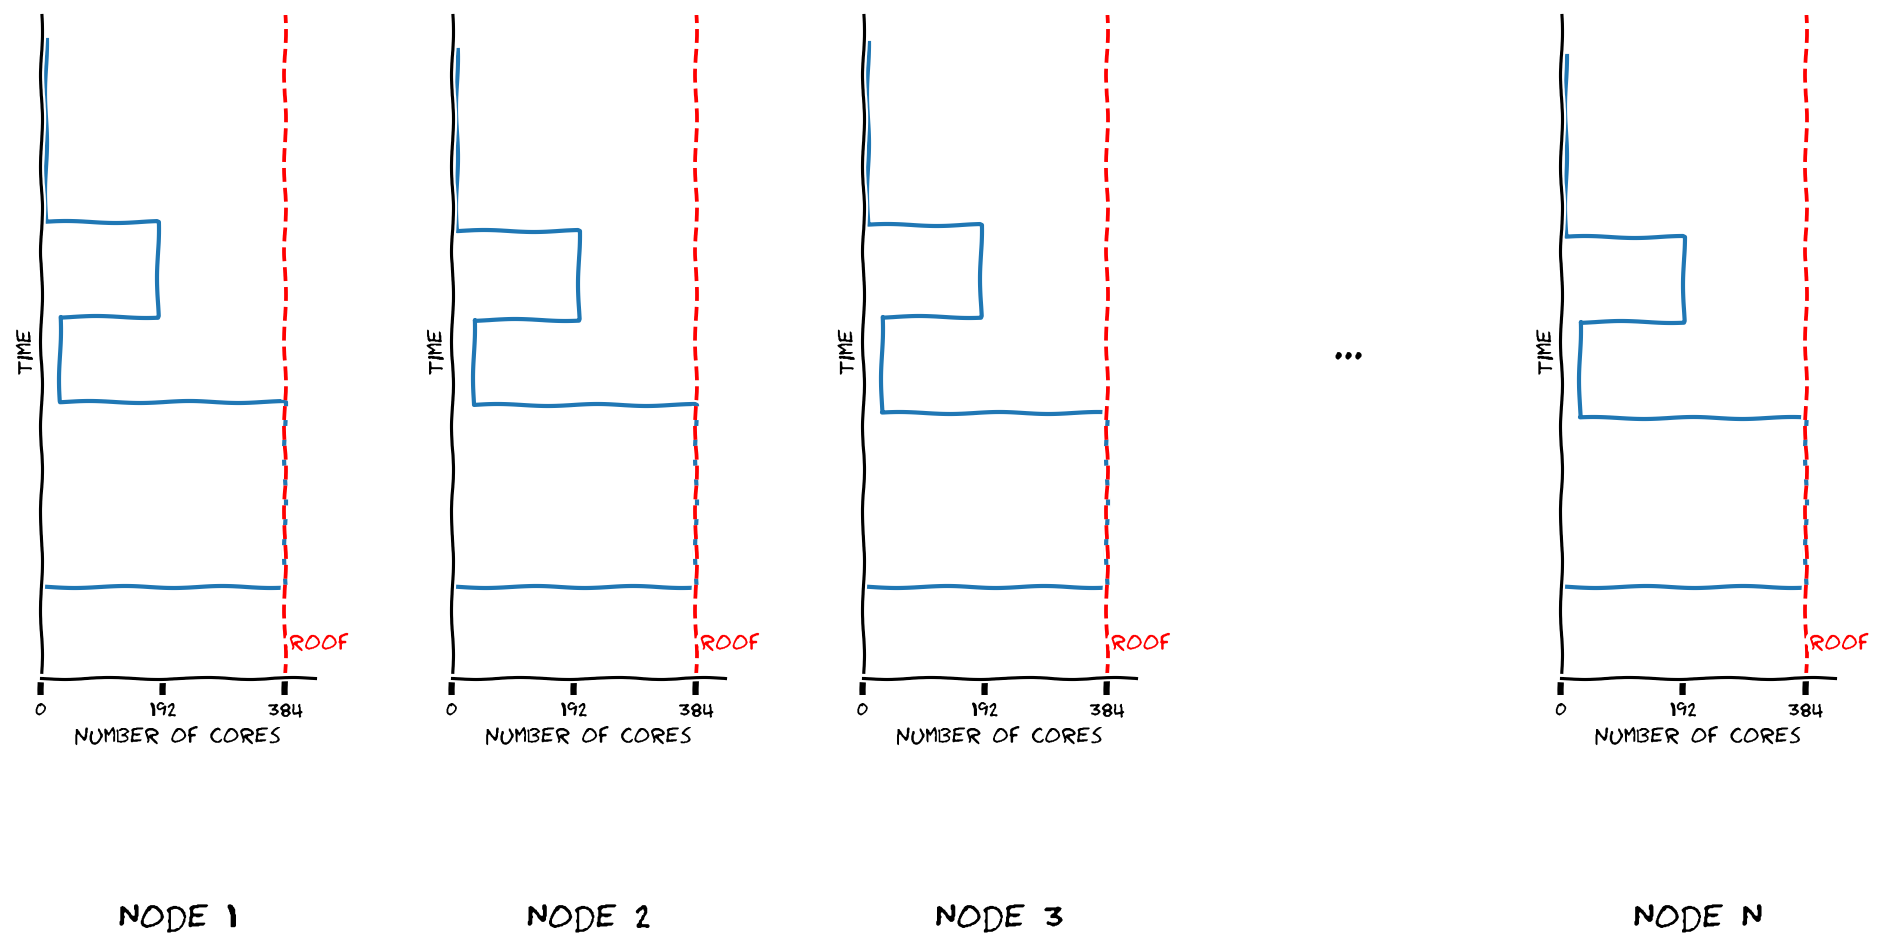
\includegraphics[width=0.9\textwidth]{efficiency/pipeline_xkcd_multinode.png}
		\end{column}
	\end{columns}
\end{frame}

%%%%%%%%%%%%%%%%%%%%%%%%%%%%%%%%%%%%%%%%%%%%%%%%%%%%%%%%%%%%%%%%%%%%%%%%%%%%%%%%
\begin{frame}
	\frametitle{Considerations II}
	\begin{columns}
		\begin{column}{0.5\textwidth}
			Assumption:
				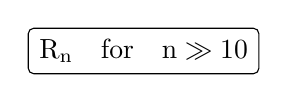
\begin{tikzpicture}
				\node[draw, rounded corners=2pt, line width=0.4pt, inner sep=4pt] {$\mathrm{R}_\mathrm{n} \quad \mathrm{for} \quad \mathrm{n} \gg 10$};
				\end{tikzpicture}
            will cause impactful random access if 
            \begin{itemize}
                \item accessed FS blocks are shared and
                \item accessed FS blocks are bigger than the file system cache.
            \end{itemize} 
		\end{column}
		\begin{column}{0.5\textwidth}
			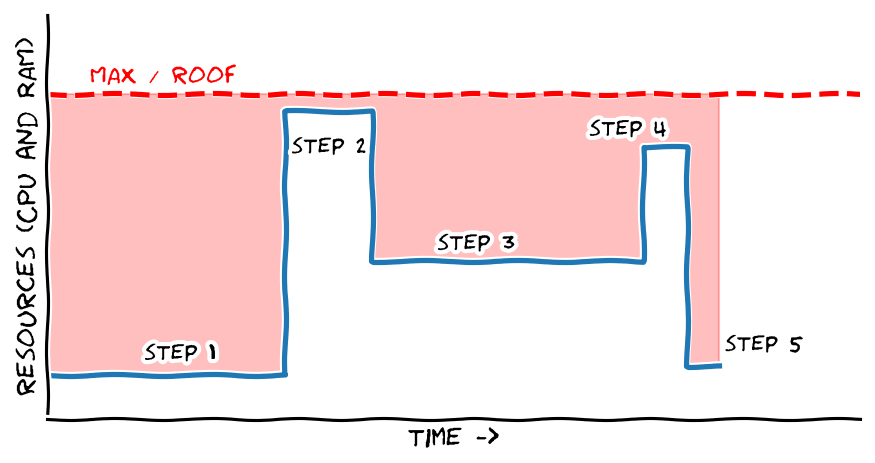
\includegraphics[width=0.9\textwidth]{efficiency/pipeline_xkcd_waste}
		\end{column}
	\end{columns}
	\pause
	\begin{hint}
		\Snakemake offers two strategies for staging files ("stage-in") - across all nodes of a job (i.\,e. for all files susceptible to random access.)
	\end{hint}
\end{frame}

%%%%%%%%%%%%%%%%%%%%%%%%%%%%%%%%%%%%%%%%%%%%%%%%%%%%%%%%%%%%%%%%%%%%%%%%%%%%%%%%
\begin{frame}
	\frametitle{Considerations III}
	\begin{columns}
		\begin{column}{0.5\textwidth}
			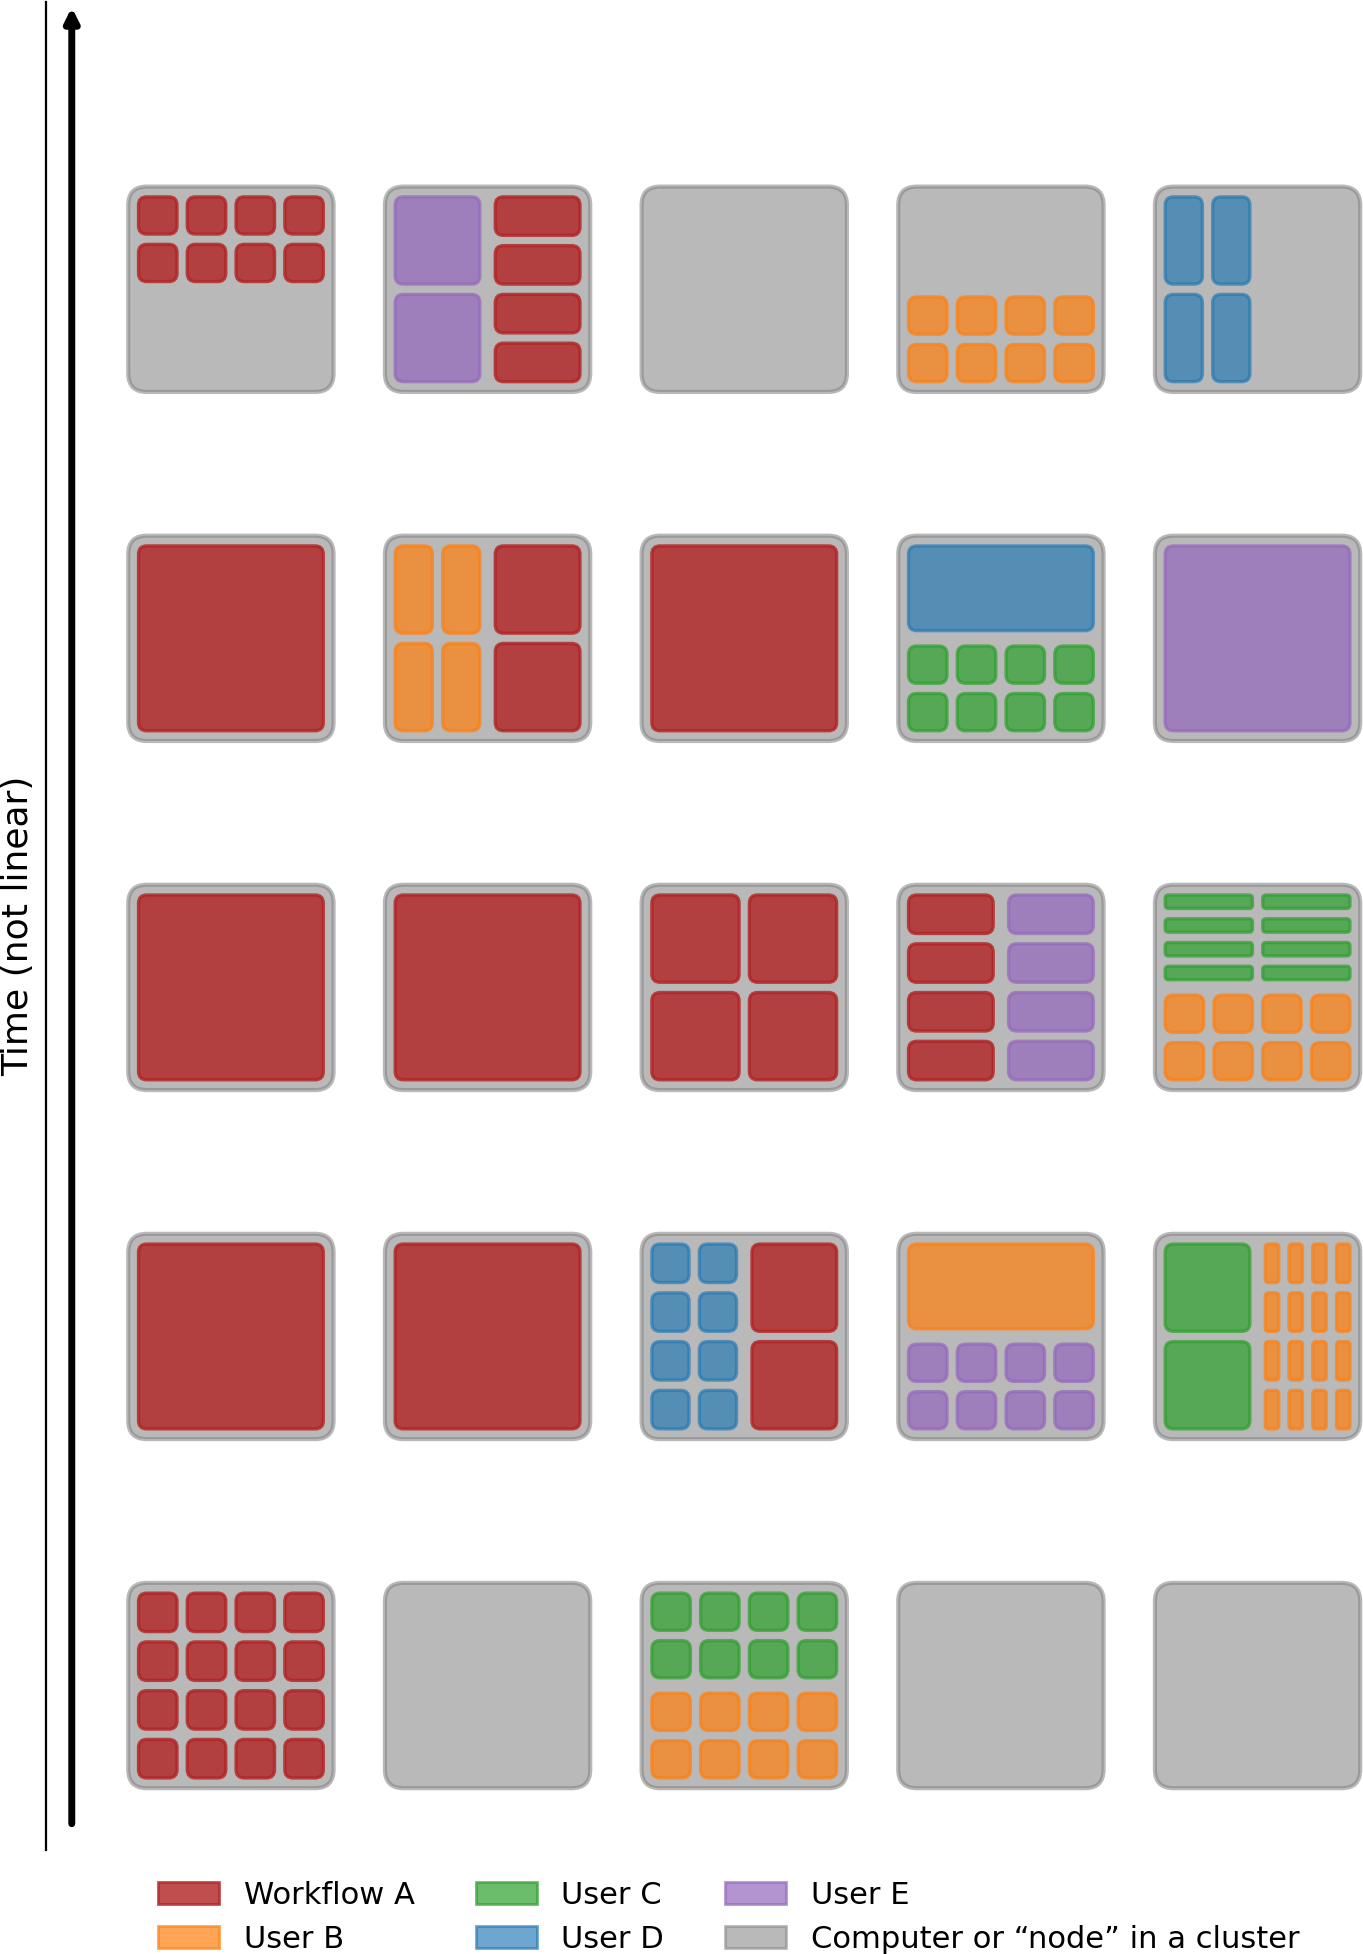
\includegraphics[width=0.7\textwidth]{efficiency/cluster_utilization}
		\end{column}
		\begin{column}{0.5\textwidth}
			Our nodes are getting bigger and bigger. The HPC -- depending on a site, of course - more and more heterogeneous
			\begin{itemize}
				\item ideal jobs (well scaling) are abundant, but not everywhere dominant
				\item even those need pre- \& post-processing
				\item Workflow Management systems offer
				\begin{itemize}
					\item to carry out small computations (plotting, download, \ldots ) on login nodes (hard to notice)
					\item to auto-select the right partition
					\item to support smp, MPI, GPU works
				\end{itemize}
			\end{itemize}
		\end{column}
	\end{columns}
\end{frame}


\subsection{Benchmarking}


%%%%%%%%%%%%%%%%%%%%%%%%%%%%%%%%%%%%%%%%%%%%%%%%%%%%%%%%%%%%%%%%%%%%%%%%%%%%%%%%%
\begin{frame}[fragile]
  \frametitle{Benchmarking for Users}
  Users can easily benchmark applications:
  \begin{lstlisting}[language=Snakemake, style=Snakemake, basicstyle=\scriptsize]
 rule foo:
   input: ...
   output: ...
   benchmark:
       "benchmark/foo/{sample}_foo.benchmark.txt"
       # or
       repeat("benchmark/foo/{sample}_foo.benchmark.txt", 3)
  \end{lstlisting}
  \pause
  %TODO: update when integrated
  \begin{docs}[Background]
  	 Benchmarking is its own subject in HPC. The \Snakemake community is actively working on \emph{optionally} gathering \& storing performance telemetry data to yield automatic best parameterization.
  \end{docs}
\end{frame}
